\section{Tensor invariants}
For a symmetric rank-2 tensor in 3D, $A_{ab} = A_{(ab)}$, there are three invariants:
\bse
\bea
I_0 &=& \det \rbm{A},\\
I_1 &=& [\rbm{A}] = {A^a}_a,\\
I_2 &=& \half  \left( [\rbm{A}]^2 - [\rbm{A}^2]\right) =\half \left( \left({A^a}_a\right)^2 - {A^a}_b{A^b}_a\right).
\eea
\ese
These invariants are the unique combinations that represent the total-derivative contractions of the matrix ${A^a}_b = \partial^a\partial_b\pi$.
Since we are in 3D, the following holds via the Cayley-Hamilton theorem
\bea
\det \rbm{A} = \frac{1}{3!}\left( [\rbm{A}]^3 - 3[\rbm{A}^2][\rbm{A}]+2[\rbm{A}^3] \right).
\eea
In $n$D there are a maximum of $n$ invariants.

We may also be interested in the invariants of rank-3 tensors in 3D; these are substantially more complicated to compute. An interesting thing to note is that  tensors which are symmetric in the last two indices, $B_{abc} = B_{a(bc)}$, are sometimes called ``peizo-electric tensors'' \cite{ahmadpeizeo}. Then the quadratic invariants are
\bea
B_{aab}B_{ccb},\qquad B_{abb}B_{acc},\qquad B_{abc}B_{abc},\qquad B_{abc}B_{bac},\qquad B_{aab}B_{bcc}
\eea
See also \url{http://www.iaeng.org/publication/WCE2013/WCE2013\_pp139-144.pdf}
\section{Relation to statistical cumulants}
Note that the tensor invariants seem related to the mean, variance, skewness, etc,  in statistics; the culumants are
\bse
\bea
\kappa_1 &=& \mu_1,\\
\kappa_2 &=& \mu_2 - \mu_1^2,\\
\kappa_3 &=& \mu_3 - 3\mu_2\mu_1 + 2\mu_1^3,\\
\kappa_4 &=& \mu_4 - 4\mu_3\mu_1 - 3 \mu_2^2 + 12\mu_2\mu_1^2 - 6\mu_1^4
\eea
\ese
And so, for the spatial 2x2 matrix ${k^a}_b$ only $\kappa_1,\kappa_2$, and $\kappa_3$ are required to specify the invariants.

\section{Symplectic current}
\subsubsection{Symplectic structure}
Suppose an action is given by the integral over a Lagrangian density which is a function of fields $q^A$ and their derivatives ${q^A}_{,i}$,
\bea
\label{eq:sec:lag-sym1-1}
\ld = \ld(q^A, {q^A}_{,i}).
\eea
A generic variation is thus given by
\bea
\delta \ld = \ld_{,A}\delta q^A + {p^i}_A\delta{q^A}_{,i},
\eea
and is easily re-writable as
\bea
\label{eq:sec:deltald}
\delta\ld =\mathcal{E}_A \delta q^A +{\vartheta^i}_{,i}
\eea
in which we defined
\bse
\bea
\label{eq:sec:symp_EA}
\mathcal{E}_A \defn    \ld_{,A} - {p^i}_{A}{}_{,i},
\eea
\bea
\label{eq:sec:symp_vthetai}
\vartheta^i \defn   {p^i}_A\delta q^A .
\eea
\ese
The ``on-shell''  dynamically permissible variations require the vanishing of (\ref{eq:sec:symp_EA}), $\mathcal{E}_A=0$. The vector (\ref{eq:sec:symp_vthetai}) is the Liouville 1-form. The pseudo-Hamiltonian density is
\bea
\mathcal{H} = {p^i}_A{q^A}_{,i} - \ld,
\eea
and whose generic variation can be expressed as
\bea
\delta\mathcal{H} = {q^A}_{,i}\delta{p^i}_{A} - \ld_{,A}\delta q^A.
\eea
For the on-shell variations (i.e., those with $\mathcal{E}_A=0$) the variation in the pseudo-Hamiltonian is
\bea
\delta\mathcal{H} = {q^A}_{,i}\delta {p^i}_A - {p^i}_{A,i} \delta q^A,
\eea
and 
\bea
\label{div_vtheta-sym}
{\vartheta^i}_{,i}=0.
\eea

Now suppose that there are two variations, $\grave{\delta}$ and $\acute{\delta}$. Then acting these onto the Lagrangian (\ref{eq:sec:lag-sym1-1}) yields
\bea
\label{eq:sec:-thouhgkjfgkf}
\grave{\delta}\acute{\delta}\ld = \mathcal{E}_A\grave{\delta}\acute{\delta}q^A +\left(\grave{\delta}  \mathcal{E}_A\right)\acute{\delta}q^A + \left( \grave{\delta}{p^i}_A \acute{\delta}q^A + {p^i}_A \grave{\delta}\acute{\delta}q^A\right)_{,i}.
\eea
Since the two variations commute
\bea
\grave{\delta}\acute{\delta}\ld = \acute{\delta}\grave{\delta}\ld
\eea
it follows from (\ref{eq:sec:-thouhgkjfgkf}) that
\bea
\label{eq:sec:sym-2form-upto}
\left(\grave{\delta}\mathcal{E}_A \right)\acute{\delta}q^A - \left(\acute{\delta}\mathcal{E}_A \right)\grave{\delta}q^A = {\widehat{\varpi} ^i}{}_{,i}
\eea
with
\bea
{\widehat{\varpi} ^i} \defn \acute{\delta}{p^i}_A \grave{\delta}q^A - \grave{\delta}{p^i}_A \acute{\delta}q^A,
\eea
which is the symplectic 2-form. For the pair of variations which are on-shell, i.e., $\mathcal{E}_A=0$, it follows from (\ref{eq:sec:sym-2form-upto}) that
\bea
\label{div_vpi-sym}
{\widehat{\varpi} ^i}{}_{,i}=0.
\eea
Rather than working with internal coordinates $i$ etc, we construct tensorial versions of the surface currents,
\bea
\Theta^{\mu} = \frac{1}{\sqrt{-\overline{g}}}{x^{\mu}}_{,i}\vartheta^i,\qquad \Omega^{\mu} = \frac{1}{\sqrt{-\overline{g}}}{x^{\mu}}_{,i}{\widehat{\varpi}^i}.
\eea
Then (\ref{div_vtheta-sym}) and (\ref{div_vpi-sym}) are expressible as
\bea
\overline{\nabla}_{\mu}\Theta^{\mu}=0,\qquad \overline{\nabla}_{\mu}\Omega^{\mu}=0.
\eea

Take
\bea
\delta\ld = \ld_{,a}\lp\phi^a + {p^{\mu}}_a\partial_{\mu}\lp \phi^a
\eea
which rearranges to
\bea
\delta \ld = \left(  \ld_{,a}- \partial_{\mu}{p^{\mu}}_a\right)\lp\phi^a + \partial_{\mu}\vartheta^{\mu},
\eea
with
\bea
\vartheta^{\mu} =   {p^{\mu}}_a\lp\phi^a .
\eea
Replacing the Lagrangian variation $\lp = \ep + \lied{\xi}$ yields
\bea
\vartheta^{\mu} =  {p^{\mu}}_a
\eea


\section{Equations of motion from a partial theory}

It is instructive to look at the variational principle as a method of constructing equations of motion. Suppose that one has a Lagrangian which contains a scalar field $\phi$, the metric $g_{\mu\nu}$, and some ``other'' field, $\qsuprm{s}{A}$, say (here ``A'' is a label, not an index). The variation of the action will yield
\bea
\label{vary-S-gen}
\delta S = \int \dd^4x\, \sqrt{-g}\, \left[ \mathcal{E}\delta\phi + \half T_{\mu\nu} \delta g^{\mu\nu} - \qsubrm{\mathcal{F}}{A}\delta\qsuprm{s}{A}\right].
\eea
It is important to note that this is the matter action and may append another action (which may also contain more terms for the scalar field, for example).
If the variation $\delta$ was generated by coordinate shifts, then the variation in the action is found from (\ref{vary-S-gen}) by replacing all instances of ``$\delta$'' by the Lie derivative $\lied{\xi}$ yielding
\bea
\delta S = \int \dd^4x\,\sqrt{-g}\,\left[ \mathcal{E} \xi^{\mu}\nabla_{\mu}\phi + T_{\mu\nu} \nabla^{(\mu}\xi^{\nu)} -  \qsubrm{\mathcal{F}}{A}\lied{\xi}\qsuprm{s}{A}\right].
\eea
This must vanish if the theory is to be diffeomorphism invariant, resulting in 
\bea
\label{eq:sec:diff-inv-conditions}
\nabla_{\mu}T^{\mu\nu} = f^{\nu}_{[\phi]} + f^{\nu}_{[s]}.
\eea
The terms on the RHS are force densities.
For this action we always have
\bea
f^{\nu}_{[\phi]} = \mathcal{E}\nabla^{\nu}\phi,
\eea
and the precise form of $f^{\nu}_{[s]}$ will depend on whether $\qsuprm{s}{A}$ is a scalar, vector, tensor, etc, field.

If $T^{\mu\nu}$ is supposed to be the energy-momentum tensor (i.e. it sits on the RHS of the Einstein equations), it must be conserved and therefore the RHS of (\ref{eq:sec:diff-inv-conditions}) must vanish. This yields the force balance condition
\bea
\label{eqq:force-balance}
f^{\nu}_{[\phi]} =- f^{\nu}_{[s]}.
\eea
As an explicit example, if $\qsubrm{s}{A} \rightarrow s$, a scalar, then 
\bea
f^{\mu}_{[s]} =   -   {\mathcal{F}}\nabla^{\mu}s.
\eea
The force balance condition (\ref{eqq:force-balance}) explicitly reads
\bea
\mathcal{E} \nabla_{\mu}\phi  =   {\mathcal{F}}\nabla_{\mu}s.
\eea
This explicitly sources the ``equation of motion'' for  the scalar $\phi$ with the field $s$.
We can rewrite this as
\bea
\mathcal{E} = \mathcal{F} \frac{\nabla^{\mu}\phi\nabla_{\mu}s}{\nabla_{\nu}\phi\nabla^{\nu}\phi}.
\eea
What we would like is for the equation of motion of the scalar  to be of the form
\bea
\mathcal{E} = \alpha\dot{\phi},
\eea
that is,
\bea
\alpha \dot{\phi} =  \mathcal{F} \frac{\nabla^{\mu}\phi\nabla_{\mu}s}{\nabla_{\nu}\phi\nabla^{\nu}\phi}.
\eea
When the fields $\phi$ and $s$ only have time-like derivatives,
\bea
\mathcal{F} = \frac{\dot{\phi}^2}{\dot{s}}\alpha.
\eea
\section{Pull-back formalism \textit{\`a la} Arkani-Hamed}
The pullback formalism we are about to discuss was developed by Arkani-Hamed et al \cite{ArkaniHamed:2001ed, ArkaniHamed:2002sp} motivated by a graph theory model for ``theory space''. They developed a method to construct an effective theory of gravity to restore coordinate invariance of linearized gravity theories. Interestingly, the pullback formalism was also laid out by Carter et al \cite{Carter26081980, Carter21111972}, more than twenty years before Arkani, during the development of relativistic elasticity theory: the mathematical language between the two motivations is identical. The Arkani-motivation was developed by the analogy with gauge field theory: there it is natural to talk of a pullback in terms of a gauge field. Infact, when numerical codes are developed, the equations of motion are discretized using a pullback and gauge field to link between lattice sites. The construction of the pullback formulation is very mathematical, but should be familiar to those who have studied differential geometry in some detail.

\subsection{Setup}

Consider a manifold, $\mathcal{U}$,  with a point on $\mathcal{U}$ being denoted by $x_{\mathcal{U}}$. Now let us have a map from the manifold to the real line:
\bea
\phi: \mathcal{U} \rightarrow \mathbb{R},
\eea
which, in a more usual notation, reads $\phi(x) \in \mathbb{R}$.
Let us also have an ``internal map''
\bea
f:\mathcal{U} \rightarrow \mathcal{U}
\eea
which is more obviously written as $x\rightarrow f(x)$. The map $\phi$ is a scalar field on $\mathcal{U}$ if it transforms under $f$ according to
\bea
\phi \rightarrow \phi\circ f.
\eea
In coordinates this reads
\bea
\phi(x) \rightarrow   \phi(f(x)).
\eea
One could think of $f$ as being a change of coordinates; later on we will give a concrete example of the map. A vector field $\rbm{A}$ on $\mathcal{U}$ transforms under $f$ according to
\bea
\rbm{A} \rightarrow \rbm{A} \circ f,
\eea
the components of $\rbm{A}$ transform as
\bea
A_{\mu}(x) \rightarrow \pd{f^{\alpha}}{x^{\mu}}(x) A_{\alpha}(f(x)).
\eea
Similarly, a tensor field
\bea
\rbm{T} \rightarrow \rbm{T}\circ f,
\eea
and its components
\bea
T_{\mu\nu}(x) \rightarrow \pd{f^{\alpha}}{x^{\mu}}(x)\pd{f^{\beta}}{x^{\nu}}(x)T_{\alpha\beta}(f(x))
\eea
This holds, for example, for the metric $\rbm{g} = g_{\mu\nu}(x) \dd x^{\mu}\otimes \dd x^{\nu}$.


Let us now introduce a second manifold, $\mathcal{V}$. This manifold is endowed with an equivalent set of maps and fields as $\mathcal{U}$. The internal map in manifold $\mathcal{V}$ is denoted as $f_{\mathcal{V}}$, so that $x_{\mathcal{V}} \rightarrow f_{\mathcal{V}}(x_{\mathcal{V}})$. In the language of Arkani, the manifolds $\mathcal{U,V}$ are two   sites of a graph connected by a link, and in the language of Carter, the manifolds contain the relaxed and strained positions of a material body. Note that we now have two manifolds and two internal transformations: $f_{\mathcal{V}}, f_{\mathcal{U}}$. We can operate each independently, but any link between the manifolds will induce some interesting structure between the transformations. This is exactly the structure we impose by including a pullback map.

Let us have a map $Y$ between these two manifolds
\bea
Y: \mathcal{U} \rightarrow \mathcal{V}.
\eea
The map between the manifolds is called a \textit{link field} in the language of Arkani.
The link field $Y (x_{\mathcal{U}})$ will associate a point $x_{\mathcal{U}}$ in $\mathcal{U}$ (the point $x_{\mathcal{U}}$ has coordinates $x^{\mu}_{\mathcal{U}}$) with a point in $\mathcal{V}$ whose coordinates are $x_{\mathcal{V}}^{\mu}  $:
\bea
Y(x_{\mathcal{U}}) = x_{\mathcal{V}}.
\eea
The link field  $Y_{\mathcal{VU}}$ is a pullback map\footnote{\textbf{Pullback} Consider  a map $F$ between two manifolds $M,W$; the map is $F:M \rightarrow W$. The manifold $M$ has coordinates $m$ and $W$ has coordinates $w$. Thus, $F(m) = w$.
Now let us have a real valued function $f$ on $W$, written as $f: W \rightarrow \mathbb{R}$.
We define the pullback of $f$ (which is on $W$) to $M$, written as $F^*f$, to be the composition $f\circ F : M \rightarrow \mathbb{R}$.
So, let us pick a point $m$ in $M$, and act the pullback on $m$. This is written as  $F^*f(m) = (f\circ F)(m) = f(F(m))$.} from $\mathcal{V}$ to $\mathcal{U}$. Under a composition of maps, the link field transforms as
\bea
Y\rightarrow f^{-1}_{\mathcal{V}} \circ Y \circ f_{\mathcal{U}},
\eea
or, in coordinates,
\bea
\label{eq:sec:trans-linkfld}
x^{\mu}_{\mathcal{V}}(x_{\mathcal{U}}) \rightarrow (f_{\mathcal{V}}^{-1})^{\mu}(Y (f_{\mathcal{U}}(x_{\mathcal{U}}))).
\eea
So, consider the object
\bea
\Psi = \psi_{\mathcal{V}} \circ Y,
\eea
where $\psi_{\mathcal{V}}$ is a scalar field in $\mathcal{V}$, then
\bea
\Psi\rightarrow  (\psi_{\mathcal{V}}\circ f_{\mathcal{V}}) \circ (f^{-1}_{\mathcal{V}} \circ Y \circ f_{\mathcal{U}}) = \psi_{\mathcal{V}} \circ Y \circ f_{\mathcal{U}} = \Psi\circ f_{\mathcal{U}} ,
\eea
i.e. $\Psi$ transforms as a scalar under the mapping in $\mathcal{U}$:
\bea
\Psi \rightarrow \Psi \circ  f_{\mathcal{U}} .
\eea
For example, the scalar field $\phi_{\mathcal{V}}(x_{\mathcal{V}})$ in $\mathcal{V}$, then
\bea
\Phi = \phi_{\mathcal{V}}\circ Y \quad\Rightarrow\quad\Phi(x_{\mathcal{U}}) = \phi_{\mathcal{V}}(Y (x_{\mathcal{U}}))
\eea 
is a scalar under $f_{\mathcal{U}}$. Similarly,
\bea
A_{\mu}(x_{\mathcal{U}}) = \pd{x_{\mathcal{V}}^{\alpha}}{x^{\mu}_{\mathcal{U}}} (x_{\mathcal{U}}) a_{\mathcal{V}\alpha}(Y (x_{\mathcal{U}})),
\eea
\bea
\label{eq:sec:trans-tensor}
T_{\mu\nu}(x_{\mathcal{U}}) = \pd{x_{\mathcal{V}}^{\alpha}}{x^{\mu}_{\mathcal{U}}} (x_{\mathcal{U}})  \pd{x_{\mathcal{V}}^{\beta}}{x^{\nu}_{\mathcal{U}}} (x_{\mathcal{U}}) t_{\mathcal{V}\alpha\beta}(Y (x_{\mathcal{U}}))
\eea
are vectors and tensors respectively under $f_{\mathcal{U}}$.
The point is, the pullback field (link field) enables the evaluation of scalar, vector, tensor etc fields in one manifold to be determined in terms of coordinates on another manifold.

\begin{figure*}[!t]
      \begin{center}
{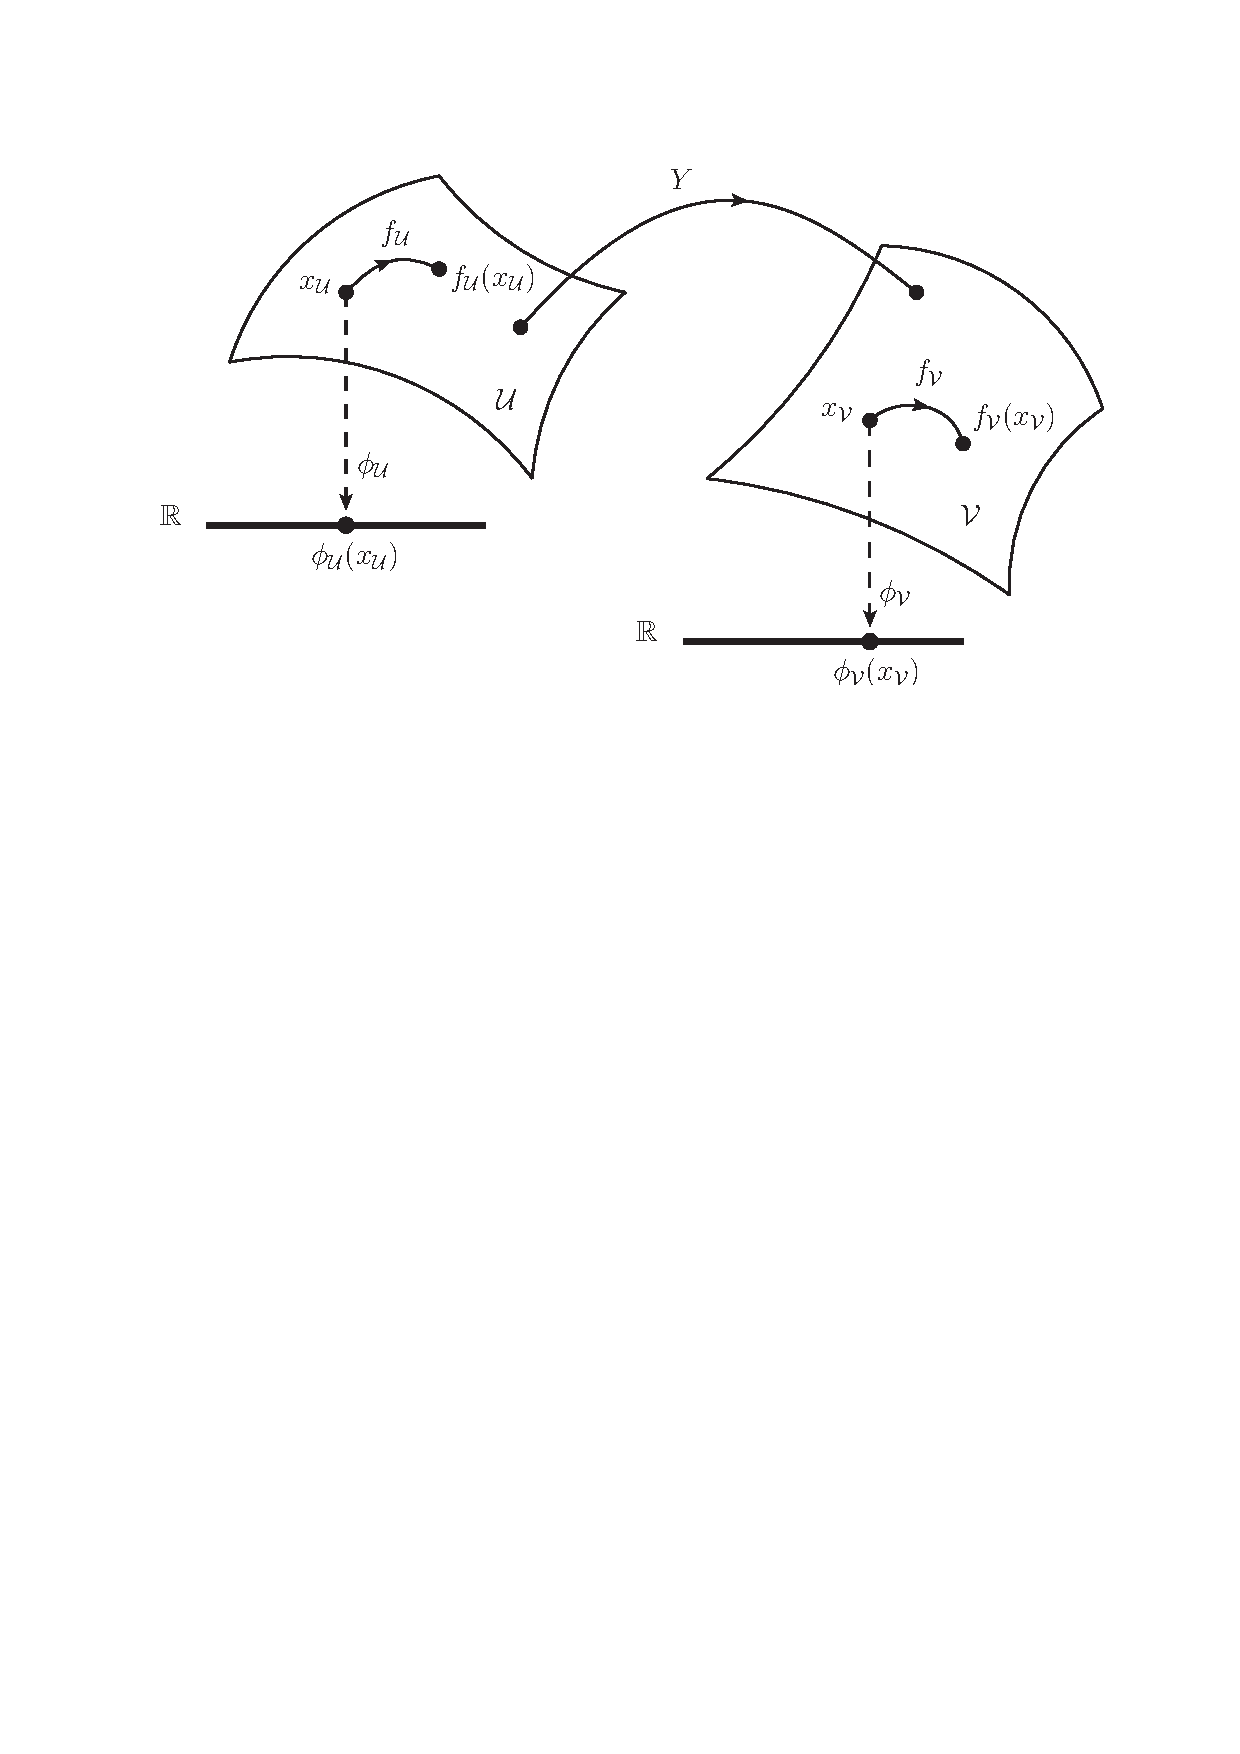
\includegraphics[scale=0.7]{images/mapping1}}
      \end{center}
\caption{The manifolds $\mathcal{U, V}$, the internal mappings $f_{\mathcal{U}}, f_{\mathcal{V}}$, the scalar field maps $\phi_{\mathcal{U}}, \phi_{\mathcal{V}}$ and the link field $Y$.} \label{fig:mapping1}
\end{figure*}

\begin{figure*}[!t]
      \begin{center}
{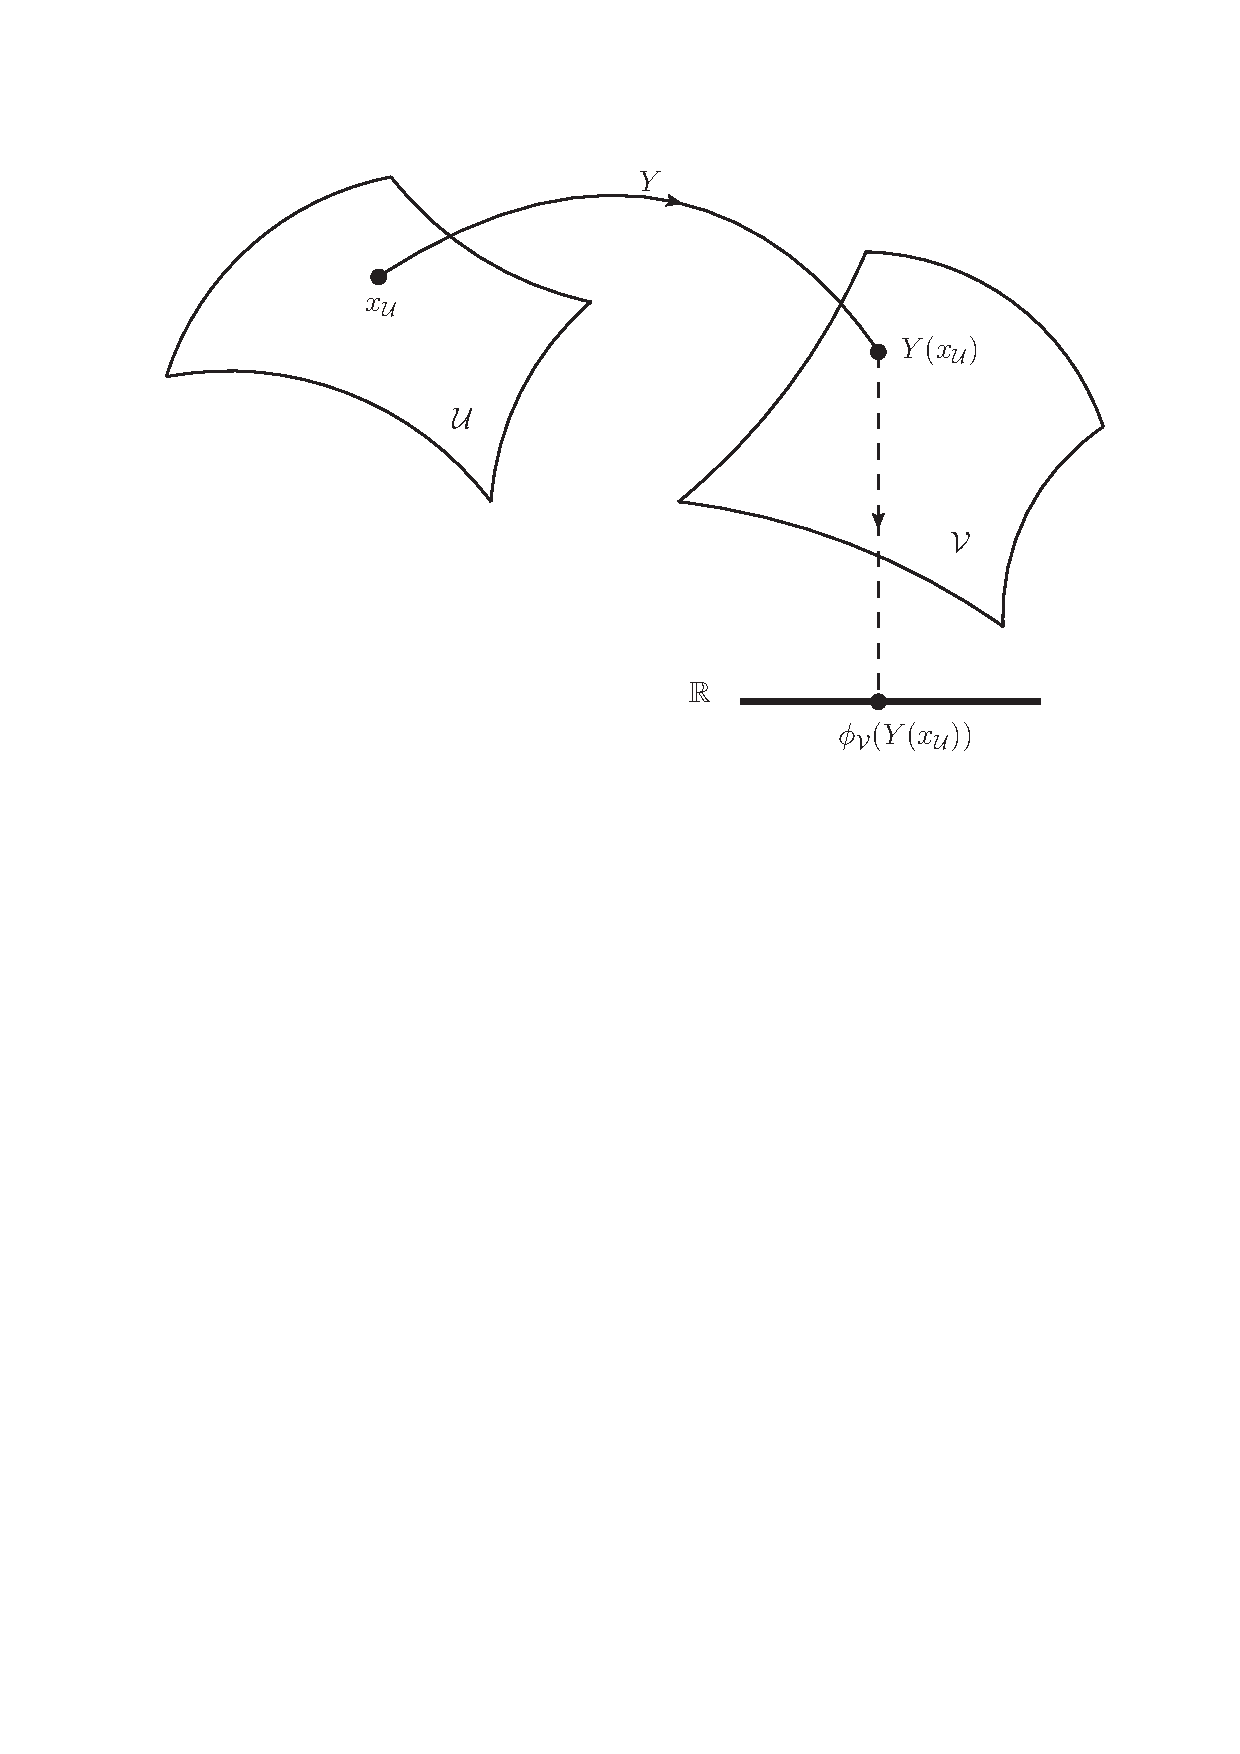
\includegraphics[scale=0.7]{images/mapping3}}
      \end{center}
\caption{The link field $Y$ maps a point $x_{\mathcal{U}}$ in $\mathcal{U}$ to a point $x_{\mathcal{V}} = Y(x_{\mathcal{U}})$ in $\mathcal{V}$. The scalar field map $\phi_{\mathcal{V}}$ in $\mathcal{V}$ then computes the value of the scalar field at that point.} \label{fig:mapping3}
\end{figure*}

\begin{figure*}[!t]
      \begin{center}
{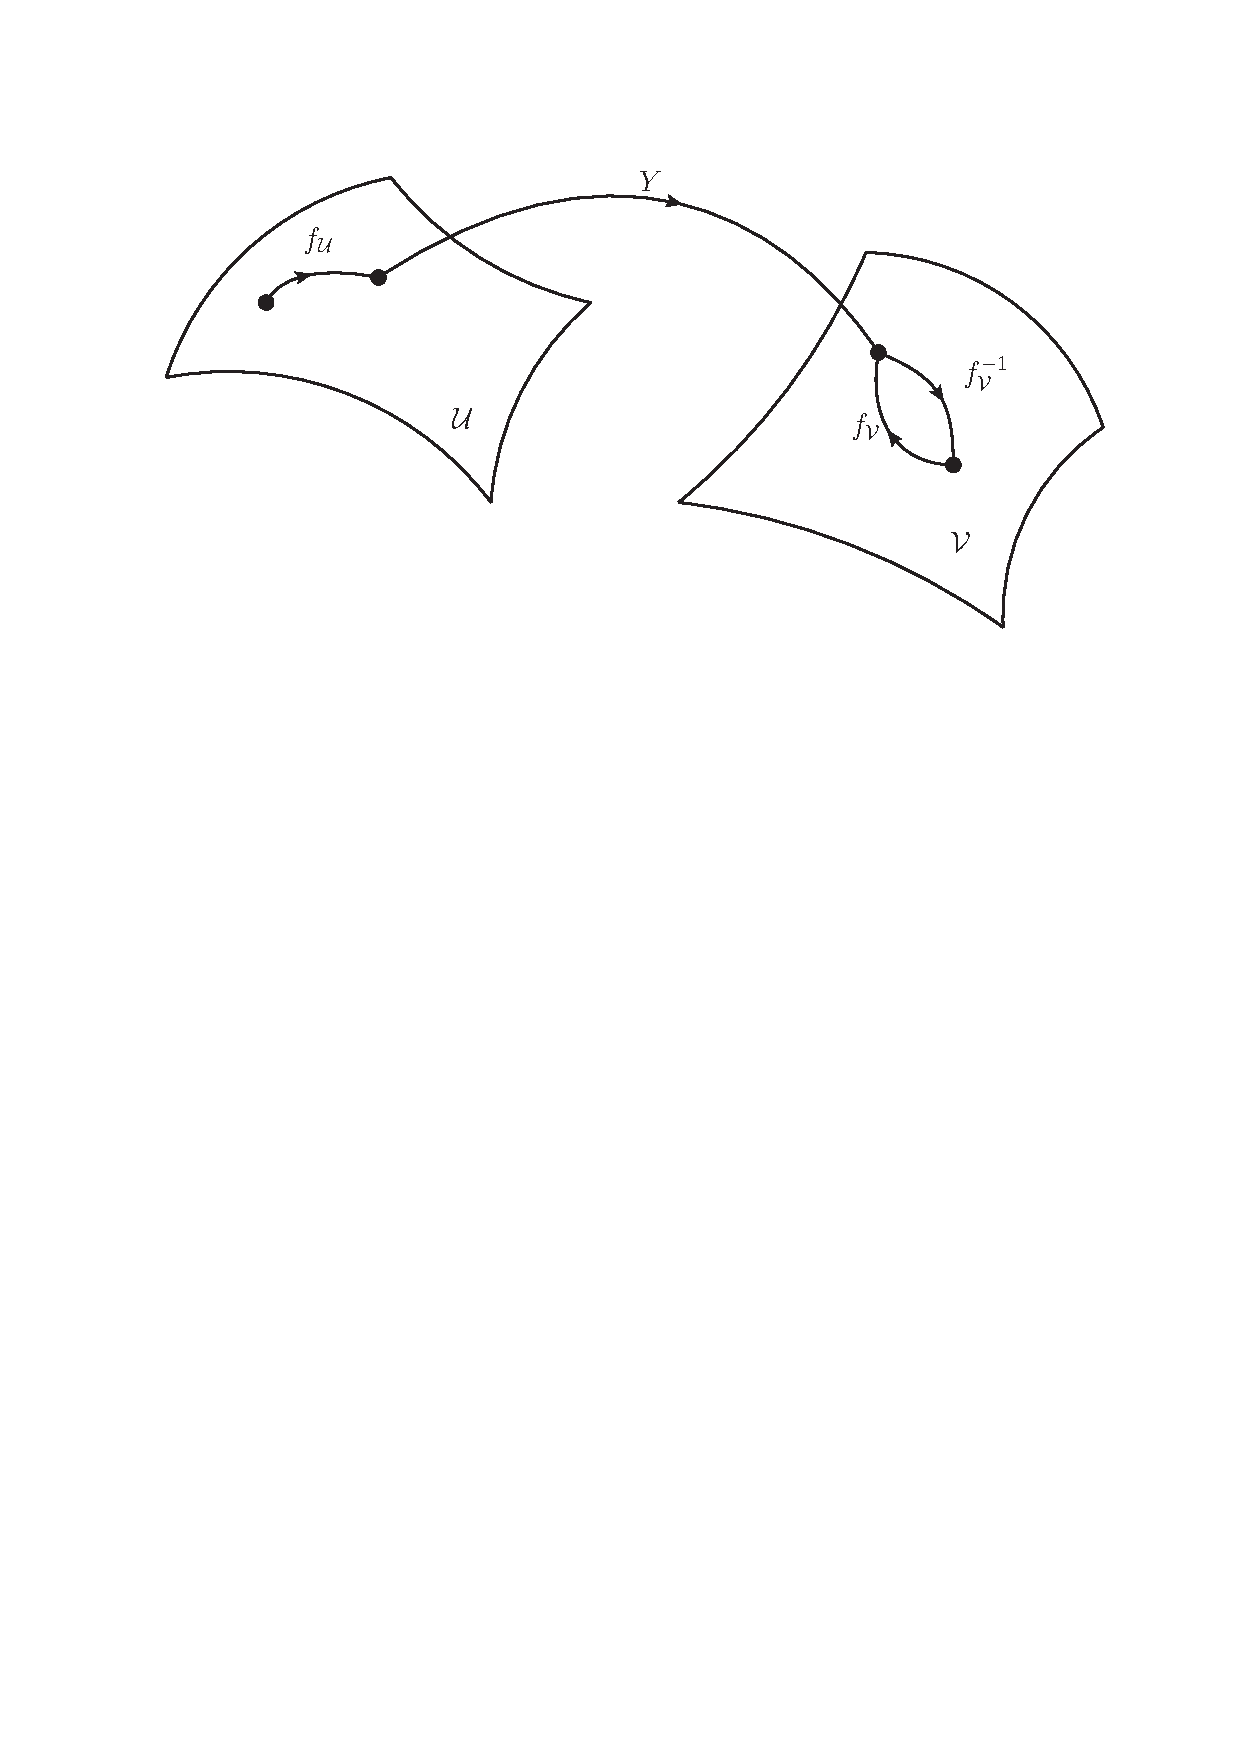
\includegraphics[scale=0.7]{images/mapping2}}
      \end{center}
\caption{The internal mapping $f_{\mathcal{U}}$ transforms between points in $\mathcal{U}$. The link field $Y$ then takes the transformed point from $\mathcal{U}$ into the transformed point in $\mathcal{V}$. The inverse mapping $f^{-1}_{\mathcal{V}}$ then finds the ``original'' point in $\mathcal{V}$ (the inverse mapping is assumed to exist).} \label{fig:mapping2}
\end{figure*}

\subsection{Studying the link field}
We will now study the link field, first in the simplest possible case, where it is the identity (also called the unitary gauge), then in the case where it is perturbatively close to the identity. We will use a deformation vector $\xi^{\mu}$ to describe the deviation of the link field from the identity. This will also describe the deviations from the unitary gauge.

In the simplest case, the link field is the identity:
\bea
\label{eq:sec:unitarygauge-link}
Y = {\rm id}\qquad \Rightarrow \qquad x_{\mathcal{V}}^{\mu} = x_{\mathcal{U}}^{\mu}.
\eea
 and the mapping between the manifolds is ``trivial''.
 
In the ``next simplest'' case the link field is perturbed away from the identity with a deformation vector, so that
\bea
\label{eq:sec:link-infitesiaml-zeta}
Y(x_{\mathcal{U}} ) = x_{\mathcal{V}} =x_{\mathcal{U}}  + \xi(x_{\mathcal{U}} )\qquad \Rightarrow \qquad x_{\mathcal{V}}^{\mu} = x_{\mathcal{U}}^{\mu} + \xi^{\mu}(x_{\mathcal{U}}).
\eea
Notice that in the unitary gauge (\ref{eq:sec:unitarygauge-link}) the deformation vector is identically zero: $\xi^{\mu}=0$. We can now insert (\ref{eq:sec:link-infitesiaml-zeta}) into (\ref{eq:sec:trans-tensor}), which we write for clarity as
\bea
T_{\mu\nu}(x_{\mathcal{U}}) &=&\bigg[ \pd{x_{\mathcal{V}}^{\alpha}(x_{\mathcal{U}})}{x^{\mu}_{\mathcal{U}}}  \bigg]\bigg[ \pd{x_{\mathcal{V}}^{\beta}(x_{\mathcal{U}}) }{x^{\nu}_{\mathcal{U}}}\bigg]\bigg[ t_{\mathcal{V}\alpha\beta}(Y_{\mathcal{VU}}(x_{\mathcal{U}}))\bigg] .
\eea
Inserting (\ref{eq:sec:link-infitesiaml-zeta}) into these terms yields
\bea
 \pd{x_{\mathcal{V}}^{\alpha}(x_{\mathcal{U}})}{x^{\mu}_{\mathcal{U}}}  = \pd{(x_{\mathcal{U}}^{\alpha} + \xi^{\alpha} )}{x^{\mu}_{\mathcal{U}}}= \delta^{\alpha}_{\mu} + \nabla_{\mu}\xi^{\alpha},
\eea
\bea
 t_{\mathcal{V}\alpha\beta}(Y_{\mathcal{VU}}(x_{\mathcal{U}})) = t_{\mathcal{V}\alpha\beta} + \xi^{\rho}\nabla_{\rho}t_{\mathcal{V}\alpha\beta} + \half \xi^{\rho}\xi^{\sigma}\nabla_{\rho}\nabla_{\sigma}t_{\mathcal{V}\alpha\beta} + \ldots
\eea
Thus, 
\bea
T_{\mu\nu}(x_{\mathcal{U}}) = t_{\mathcal{V}\mu\nu} + \xi^{\rho}\nabla_{\rho}t_{\mathcal{V}\mu\nu}+ 2 t_{\mathcal{V}\alpha(\mu}\nabla_{\nu)}\xi^{\alpha} + \ldots.
\eea
All terms on the right-hand-side are functions of $x_{\mathcal{U}}$. The series continues in quadratic and higher powers of the vector $\xi^{\mu}$. By our initial construction, $T_{\mu\nu}(x_{\mathcal{U}})$ transforms as a tensor in $\mathcal{U}$ under $f_{\mathcal{U}}$. The second term on the RHS will vanish when $t_{\mathcal{V}\mu\nu}$ is taken to be the metric. We will call $\xi^{\mu}$ the deformation vector. In Arkani-Hamed et al \cite{ArkaniHamed:2002sp} the $\xi^{\mu}$ are called Goldstone fields, and they find it instructive to write the Goldstone field in ``pion'' notation $\xi \equiv\pi$, and decompose the pion field
\bea
\pi_{\mu} = A_{\mu} + \nabla_{\mu}\sigma,
\eea
where $\nabla_{\mu}A^{\mu}=0$. The Goldstone pions enable an interesting discussion of massive gravity theories to take place, where, for example, the   $\sigma$-field has a ghost, unless the Pauli-Feirz mass term is used. The fields $\{\pi, A, \sigma\}$ are called Stuckleberg fields \cite{Green1991462}.
\subsection{The internal transformation is a coordinate shift}
Now suppose that the internal transformation $f$ is a shift in position:
\bea
 x_{\mathcal{U}} \rightarrow  f_{\mathcal{U}} ( x_{\mathcal{U}} ),\qquad f_{\mathcal{U}}(x_{\mathcal{U}}) = x_{\mathcal{U}} + \epsilon_{\mathcal{U}}(x_{\mathcal{U}}).
\eea
Similarly,
\bea
f_{\mathcal{V}}(x_{\mathcal{V}}) = x_{\mathcal{V}} + \epsilon_{\mathcal{V}}(x_{\mathcal{V}})
\eea

Under this coordinate transformation,
\bea
T_{\mu\nu}(x_{\mathcal{U}})\rightarrow T_{\mu\nu}(x_{\mathcal{U}} + \epsilon_{\mathcal{U}}) = T_{\mu\nu}(x_{\mathcal{U}}) + \lied{\epsilon_{\mathcal{U}}}T_{\mu\nu} ,
\eea
where the Lie derivative is
\bea
\lied{\epsilon_{\mathcal{U}}}T_{\mu\nu}  = \epsilon^{\alpha}_{\mathcal{U}}\nabla_{\alpha}T_{\mu\nu} + 2T_{\alpha(\mu}\nabla_{\nu)}\epsilon^{\alpha}_{\mathcal{U}}.
\eea
Thus, we say that under the   transformation $f_{\mathcal{U}}$ we have, $T_{\mu\nu}(x_{\mathcal{U}})\rightarrow T_{\mu\nu}(x_{\mathcal{U}}) + \delta T_{\mu\nu}(x_{\mathcal{U}})$ where
\bea
\delta T_{\mu\nu}(x_{\mathcal{U}}) = \epsilon^{\alpha}_{\mathcal{U}}\nabla_{\alpha}T_{\mu\nu} + 2T_{\alpha(\mu}\nabla_{\nu)}\epsilon^{\alpha}_{\mathcal{U}}.
\eea
Similarly, under $f_{\mathcal{V}}$,
\bea
\delta t_{\mu\nu}(x_{\mathcal{V}}) = \epsilon^{\alpha}_{\mathcal{V}}\nabla_{\alpha}t_{\mu\nu} + 2t_{\alpha(\mu}\nabla_{\nu)}\epsilon^{\alpha}_{\mathcal{V}}.
\eea
By using (\ref{eq:sec:trans-linkfld})  we see that under the   transformation $f_{\mathcal{U}}$ the link field transforms into
\bea
Y( x_{\mathcal{U}}) \rightarrow Y(f_{\mathcal{U}}(x_{\mathcal{U}}))
\eea
where 
\bea
Y(f_{\mathcal{U}}(x_{\mathcal{U}})) &=& Y(x_{\mathcal{U}} + \epsilon_{\mathcal{U}}(x_{\mathcal{U}})) \nonumber\\
&=& x_{\mathcal{U}} + \epsilon_{\mathcal{U}}(x_{\mathcal{U}}) + \xi(x_{\mathcal{U}} + \epsilon_{\mathcal{U}}(x_{\mathcal{U}}))\nonumber\\
&=& x_{\mathcal{U}} + \epsilon_{\mathcal{U}}(x_{\mathcal{U}}) + \xi(x_{\mathcal{U}}) + \epsilon_{\mathcal{U}}^{\mu}\nabla_{\mu}\xi\nonumber\\
&=&  x_{\mathcal{U}} +   \xi  + \delta\xi,
\eea
where
\bea
\delta\xi^{\mu} = \epsilon^{\mu}_{\mathcal{U}}  + \epsilon_{\mathcal{U}}^{\alpha}\nabla_{\alpha}\xi^{\mu} .
\eea
Thus, we have established how the deformation vector (Goldstone boson) shifts under an infinitesimal coordinate transformation $f_{\mathcal{U}}$.

Now, because $f_{\mathcal{V}}(x) = x + \epsilon_{\mathcal{V}}(x)$, and $f_{\mathcal{V}}^{-1}\circ f_{\mathcal{V}} = {\rm id}$ by definition, we can obtain
\bea
f_{\mathcal{V}}^{-1}(x) = x - \epsilon_{\mathcal{V}}(x).
\eea
We now check that this inverse function   satisfies the required property:
\bea
f_{\mathcal{V}}^{-1}\circ f_{\mathcal{V}}(x)  = f_{\mathcal{V}}^{-1}(x + \epsilon_{\mathcal{V}}(x)) = (x + \epsilon_{\mathcal{V}}(x)) - \epsilon_{\mathcal{V}}(x) = x = {\rm id}.
\eea
Now, from (\ref{eq:sec:trans-linkfld})
\bea
Y(x_{\mathcal{U}}) \rightarrow f_{\mathcal{V}}^{-1} (Y_{\mathcal{VU}}(f_{\mathcal{U}}(x_{\mathcal{U}}))) = f^{-1}_{\mathcal{V}}(Y) = Y - \epsilon_{\mathcal{V}}(Y).
\eea
So, under $f_{\mathcal{V}}$,
\bea
Y \rightarrow Y - \epsilon_{\mathcal{V}}(Y)&=&x + \xi - \epsilon_{\mathcal{V}}(x + \xi) \nonumber\\
&=& x + \xi - \epsilon_{\mathcal{V}} - \xi^{\alpha}\nabla_{\alpha}\epsilon_{\mathcal{V}} - \half \xi^{\alpha}\xi^{\beta} \nabla_{\alpha}\nabla_{\beta}\epsilon_{\mathcal{V}} + \ldots\nonumber\\
&=& x+\xi + \delta \xi,
\eea
where
\bea
\delta \xi^{\mu} = - \epsilon^{\mu}_{\mathcal{V}}(x + \xi) = - \epsilon^{\mu}_{\mathcal{V}} - \xi^{\alpha}\nabla_{\alpha}\epsilon_{\mathcal{V}}^{\mu} - \half \xi^{\alpha}\xi^{\beta} \nabla_{\alpha}\nabla_{\beta}\epsilon_{\mathcal{V}}^{\mu} + \ldots
\eea
Now we have an expression for how the deformation vector transforms under   the internal transformations $f_{\mathcal{U}}$ and $f_{\mathcal{V}}$:
\bea
\delta \xi^{\mu} =  \epsilon^{\mu}_{\mathcal{U}}  - \epsilon^{\mu}_{\mathcal{V}} + \epsilon_{\mathcal{U}}^{\alpha}\nabla_{\alpha}\xi^{\mu}  - \xi^{\alpha}\nabla_{\alpha}\epsilon_{\mathcal{V}}^{\mu} - \half \xi^{\alpha}\xi^{\beta} \nabla_{\alpha}\nabla_{\beta}\epsilon_{\mathcal{V}}^{\mu} + \ldots
\eea

Under $f_{\mathcal{V}}$,
\bea
\delta T_{\mu\nu} = \delta t_{\mu\nu} + \xi^{\rho}\nabla_{\rho}\delta t_{\mu\nu} + 2 \delta t_{\alpha(\mu}\nabla_{\nu)}\xi^{\alpha} + \delta\xi^{\rho}\nabla_{\rho}t_{\mu\nu} + 2 t_{\alpha(\mu}\nabla_{\nu)}\delta \xi^{\alpha}
\eea
\subsection{Example: massive gravity}



As an example, we could take the tensor field to be the metric, in which case
\bea
h_{\mu\nu} = g_{\mu\nu} -   \pd{x_{\mathcal{V}}^{\alpha} }{x^{\mu}_{\mathcal{U}}}   \pd{x_{\mathcal{V}}^{\beta}  }{x^{\nu}_{\mathcal{U}}}\bar{g}_{\alpha\beta}(Y_{\mathcal{VU}}(x_{\mathcal{U}})) .
\eea
After using  the link field $Y(x) = x - \xi$, and writing ${\tt h} = g - \bar{g}$,
\bea
h_{\mu\nu} = {\tt h}_{\mu\nu} + 2 \nabla_{(\mu}\xi_{\nu)}.
\eea
The deformation vector can be decomposed into a scalar piece and a divergence-less vector:
\bea
\label{eq:sec:massive-gravition-expsn}
h_{\mu\nu} = {\tt h}_{\mu\nu} + 2\nabla_{(\mu}A_{\nu)} + 2 \nabla_{\mu}\nabla_{\nu}\sigma.
\eea
A generic mass term in the action will be
\bea
\label{eq:sec:genmassterm-massgrav}
S \supset\qsubrm{S}{mass} = \int_M \mathcal{W}^{\mu\nu\alpha\beta} h_{\mu\nu}h_{\alpha\beta},
\eea
and so will contain terms such as
\bea
{\tt h}^2,\quad {\tt h}\nabla A,\quad \nabla A\nabla A,\quad {\tt h}\nabla\nabla\sigma,\quad \nabla A\nabla\nabla\sigma,\quad \nabla\nabla\sigma\nabla\nabla\sigma.
\eea
These second derivative terms of the $\sigma$-field in the Lagrangian will generically produce ghosts, unless the way in which they are contracted made them vanish. Arkani observes that the combination of the coefficients that is required to make these terms vanish  gives rise to the Pauli-Feirz term, $h^{\mu\nu}h_{\mu\nu} - h^2$. The Pauli-Feirz mass-tensor is
\bea
\label{eq:sec:pauli-feirz-mass-tensor}
 {\mathcal{W}}_{\rm\scriptscriptstyle (PF)}^{\mu\nu\alpha\beta} = g^{\mu(\alpha}g^{\beta)\nu} - g^{\mu\nu}g^{\alpha\beta}.
\eea

\section{Multi-constituent fluids}
Here we review Carter's construction \cite{carter_springer_cond}. See also \cite{1991Carter_12}, \cite{LopezMonsalvo:2010ut}, \cite{PhysRevD.43.1223}

Suppose there are a set of currents, $\qsubrm{n}{X}^{\mu}$; here, the subscript ``X'' is a constituent index, and when they are repeated they are assumed to be summed over (unless explicitly stated). In the material space, the variation of the master function $\Lambda$ is
\bea
\dd \Lambda = \pd{\Lambda}{\gamma_{IJ}}\dd \gamma_{IJ} + \pd{\Lambda}{{^{\perp}\qsubrm{n}{X}^I}}\dd ^{\perp}\qsubrm{n}{X}^I + \pd{\Lambda}{\qsubrm{n}{X}^{//}}\dd \qsubrm{n}{X}^{//}.
\eea
The convective derivative in terms of space-time fields is thus
\bea
\qsubrm{\dd}{C}\Lambda &=& \pd{\Lambda}{\gamma_{\mu\nu}}\qsubrm{\dd}{C} \gamma_{\mu\nu} + \pd{\Lambda}{{^{\perp}\qsubrm{n}{X}^{\mu}}}\qsubrm{\dd}{C} ^{\perp}\qsubrm{n}{X}^{\mu} + \pd{\Lambda}{\qsubrm{n}{X}^{//}}\qsubrm{\dd}{C} \qsubrm{n}{X}^{//}.
\eea
We can bring the longitudinal and orthogonal projective pieces together and write
\bea
\label{eq:sec:var-L-mixed-all-dlsghfkhsg}
\qsubrm{\dd}{C}\Lambda =  \pd{\Lambda}{\gamma_{\mu\nu}}\qsubrm{\dd}{C} \gamma_{\mu\nu} +\pd{\Lambda}{\qsubrm{n}{X}^{\mu}}\qsubrm{\dd}{C}\qsubrm{n}{X}^{\mu}
\eea
in which
\bea
\pd{\Lambda}{\qsubrm{n}{X}^{\mu}} =  \pd{\Lambda}{{^{\perp}\qsubrm{n}{X}^{\mu}}}- u_{\mu}\pd{\Lambda}{\qsubrm{n}{X}^{//}}.
\eea
with
\bea
\label{eq:sec:decmp_n}
{^{\perp}\qsubrm{n}{X}^{\mu}} = {\gamma^{\mu}}_{\nu}\qsubrm{n}{X}^{\nu},\qquad \qsubrm{n}{X}^{//} = - u_{\mu}\qsubrm{n}{X}^{\mu}.
\eea
The Lagrangian variation is then given by
\bea
\qsubrm{\dd}{L} \Lambda = \qsuprm{\chi}{X}_{\mu}\qsubrm{\dd}{L} \qsubrm{n}{X}^{\mu} + \pd{\Lambda}{g_{\mu\nu}} \qsubrm{\dd}{L} g_{\mu\nu},
\eea
in which the momentum covectors are
\bse
\bea
\qsuprm{\chi}{X}_{\mu} = \pd{\Lambda}{\qsubrm{n}{X}^{\mu}},
\eea
and
\bea
\label{pdLg}
\pd{\Lambda}{g_{\mu\nu}} = \pd{\Lambda}{\gamma_{\mu\nu}} - u^{\rho}\qsuprm{\chi}{X}_{\rho}\qsubrm{n}{X}^{\sigma}\left({\gamma^{(\mu}}_{\sigma}u^{\nu)} - \tfrac{1}{2}u_{\sigma}u^{\mu}u^{\nu}\right).
\eea
\ese
The momentum covectors $\qsuprm{\chi}{X}_{\mu}$ can be decomposed in a physically intuitive manner as
\bea
\qsuprm{\chi}{X}_{\mu}  = \qsuprm{\mu}{X}u_{\mu} + \qsuprm{p}{X}_{\mu},
\eea
where the effective inertia $\qsuprm{\mu}{X}$ and 3-momentum $ \qsuprm{p}{X}_{\mu}$ are given by
\bea
\qsuprm{\mu}{X} =- \pd{\Lambda}{\qsubrm{n}{X}^{//}},\qquad \qsuprm{p}{X}_{\mu} =  \pd{\Lambda}{{^{\perp}\qsubrm{n}{X}^{\mu}}}.
\eea

The variations of all quantities have two origins. The first is Eulerian variation, $\qsubrm{\dd}{E}$, which is variation with respect to the gravitational background. Secondly there are variations due to displacements of the world-lines of the flow. These are produced by $\xi^{\mu}$ which is displacement of the flow, and $\qsubrm{\xi}{X}^{\mu}$ for independent displacements of the world-lines of each constituent of the substance. This all translates into the following expressions for the Lagrangian variation of the metric and currents,
\bse
\bea
\qsubrm{\dd}{L}g_{\mu\nu} = \qsubrm{\dd}{E}g_{\mu\nu} + 2 \nabla_{(\mu}\xi_{\nu)},
\eea
\bea
\qsubrm{\dd}{L} \qsubrm{n}{X}^{\mu} = - \qsubrm{n}{X}^{\mu}\left( \nabla_{\nu}\qsubrm{\eta}{\{X\}}^{\nu} + \tfrac{1}{2}g^{\alpha\beta}\qsubrm{\dd}{L}g_{\alpha\beta}\right) + \qsubrm{n}{X}^{\nu}\nabla_{\nu}\qsubrm{\eta}{\{X\}}^{\mu} - \qsubrm{\eta}{\{X\}}^{\nu}\nabla_{\nu}\qsubrm{n}{X}^{\mu},
\eea
\ese
in which $\qsubrm{\eta}{X}^{\mu}$ represents the difference between the wordline displacement of each constituent
\bea
\qsubrm{\eta}{X}^{\mu} = \qsubrm{\xi}{X}^{\mu} - \xi^{\mu},
\eea
and where the curly-braces are used to exclude the use of summations over the constituent indices. The Eulerian variation of the currents can be written as
\bea
\qsubrm{\dd}{E} \qsubrm{n}{X}^{\mu} = - \half \qsubrm{n}{X}^{\mu}g^{\alpha\beta}\qsubrm{\dd}{E}g_{\alpha\beta} + \qsubrm{n}{X}^{\nu}\nabla_{\nu}\qsubrm{\xi}{\{X\}}^{\mu} - \nabla_{\nu}\left( \qsubrm{n}{X}^{\mu}\qsubrm{\xi}{\{X\}}^{\nu}\right).
\eea
Putting this together, we arrive at the measure-weighted Eulerian variation of the master function,
\bea
\frac{1}{\sqrt{-g}}\qsubrm{\dd}{E}\left( \sqrt{-g}\Lambda\right) = \half T^{\mu\nu} \qsubrm{\dd}{E}g_{\mu\nu} + f_{\mu}\xi^{\mu} + \qsuprm{f}{X}_{\mu}\qsubrm{\xi}{X}^{\mu} + \nabla_{\mu}S^{\mu},
\eea
in which the energy-momentum tensor is given by
\bea
\label{eq:sec:emt-multi-fluid}
T^{\mu\nu} = 2\pd{\Lambda}{g_{\mu\nu}} + \left(\Lambda - \qsuprm{\chi}{X}_{\sigma}\qsubrm{n}{X}^{\sigma}\right)g^{\mu\nu},
\eea
the individual forces are
\bea
\label{eq:fx-defn-cart}
\qsuprm{f}{X}_{\mu} = \qsuprm{\chi}{X}_{\mu}\nabla_{\nu}\qsubrm{n}{\{X\}}^{\nu} + 2 \qsubrm{n}{\{X\}}^{\nu}\nabla_{[\nu}\qsuprm{\chi}{X}_{\mu]},
\eea
the self-force is
\bea
f_{\mu} = \nabla_{\nu}{T^{\nu}}_{\mu} - \sum_{\rm{X}} \qsuprm{f}{X}_{\mu},
\eea
and the total derivative current is given by
\bea
S^{\mu} \defn \left( T^{\mu\nu} - \Lambda g^{\mu\nu}\right)\xi_{\nu} + 2 \qsubrm{n}{\{X\}}^{[\mu}\qsubrm{\eta}{X}^{\nu]} \qsuprm{\pi}{X}_{\nu}.
\eea
By recalling (\ref{pdLg}), the energy-momentum tensor (\ref{eq:sec:emt-multi-fluid}) can be written  in a more conventional manner, where we isolate the energy density, flux, and pressure tensor as
\bea
T^{\mu\nu} = \rho u^{\mu}u^{\nu} + 2 Q^{(\mu}u^{\nu)} + P^{\mu\nu},
\eea
with
\bse
\bea
\rho = {^{\perp}\qsubrm{n}{X}}\qsuprm{p}{X}_{\mu} - \Lambda,
\eea
\bea
\label{eq:sec:emt_heatflux}
Q^{\mu} = \qsuprm{\mu}{X} {}^{\perp}\qsubrm{n}{X}^{\mu},
\eea
\bea
P^{\mu\nu} = 2\pd{\Lambda}{\gamma_{\mu\nu}} + \left( \Lambda - \qsuprm{\chi}{X}_{\sigma}\qsubrm{n}{X}^{\sigma}\right)\gamma^{\mu\nu}.
\eea
\ese
\subsection{Two constituent model}
\begin{itemize}
\item Two constituent fluid was studied in \cite{LopezMonsalvo:2010ut}, and the cosmology in \cite{Comer:2011ss} (although that was just at the background)
\end{itemize}

Let us expose all formulae in the two-constituent model. The particle currents are
\bea
\qsubrm{n}{0}^{\mu} = s^{\mu},\qquad \qsubrm{n}{1}^{\mu} = n^{\mu},
\eea
and the momentum covectors are
\bea
\qsuprm{\chi}{0}_{\mu} = \theta_{\mu},\qquad \qsuprm{\chi}{1}_{\mu} = \chi_{\mu}.
\eea
We also assume covariance, which means that the master function is a function of scalars formed out of all particle currents:
\bea
\Lambda =  \Lambda (n,s,j),
\eea
where
\bea
n = (-n_{\mu}n^{\mu})^{1/2},\qquad s = (-s_{\mu}s^{\mu})^{1/2},\qquad j =  (-n_{\mu}s^{\mu})^{1/2}.
\eea
Notice that $j$ quantifies the leaking between the currents (also known as entrainment). The convective derivative of the master function (\ref{eq:sec:var-L-mixed-all-dlsghfkhsg}) now reads
\bea
\qsubrm{\dd}{C}\Lambda =\pd{\Lambda}{\gamma_{\mu\nu}}\qsubrm{\dd}{C}\gamma_{\mu\nu}+ \pd{\Lambda}{n^{\mu}}\qsubrm{\dd}{C} n^{\mu} + \pd{\Lambda}{s^{\mu}}\qsubrm{\dd}{C}s^{\mu},
\eea
in which
\bse
\bea
\pd{\Lambda}{\gamma_{\mu\nu}} = - \frac{1}{2n}\pd{\Lambda}{n} n^{\mu}n^{\nu}- \frac{1}{2s}\pd{\Lambda}{s} s^{\mu}s^{\nu}  - \frac{1}{2j}\pd{\Lambda}{j}n^{\mu}s^{\nu},
\eea
\bea
\pd{\Lambda}{n^{\mu}} =-\frac{1}{n} \pd{\Lambda}{n}n_{\mu} - \frac{1}{2j}\pd{\Lambda}{j}s_{\mu},
\eea
\bea
\pd{\Lambda}{s^{\mu}} =-\frac{1}{s} \pd{\Lambda}{s}s_{\mu} - \frac{1}{2j}\pd{\Lambda}{j}n_{\mu}.
\eea
\ese
Hence, the Lagrangian variation of the master function is
\bea
\qsubrm{\dd}{L}\Lambda = \pd{\Lambda}{g_{\mu\nu}}\qsubrm{\dd}{L} g_{\mu\nu}+ \chi_{\mu}\qsubrm{\dd}{L} n^{\mu}  + \theta_{\mu}\qsubrm{\dd}{L} s^{\mu} ,
\eea
where we read off the expressions for the momentum covectors,
\bse
\bea
\chi_{\mu} \defn \pd{\Lambda}{n^{\mu}} = g_{\mu\nu} \left( \qsuprm{B}{n}n^{\nu} + Cs^{\nu}\right),
\eea
\bea
\theta_{\mu} = \pd{\Lambda}{s^{\mu}} = g_{\mu\nu} \left( \qsuprm{B}{s}s^{\nu} + Cn^{\nu}\right),
\eea
\ese
where the cofficients are
\bea
\qsuprm{B}{n} \defn -\frac{1}{n}\pd{\Lambda}{n},\qquad \qsuprm{B}{s} \defn -\frac{1}{s}\pd{\Lambda}{s},\qquad C \defn - \frac{1}{2j}\pd{\Lambda}{j}.
\eea
We now work in the matter frame and pick $n^{\mu}$ to be parallel to $u^{\mu}$,
\bea
n^{\mu} = n u^{\mu},
\eea
and set
\bea
s^{\mu} = s^\star(u^{\mu} + w^{\mu}),
\eea
with $u^{\mu}w_{\mu}=0$. Hence, the momenta are
\bse
\bea
\chi_{\mu} = \left(\qsuprm{B}{n} n + Cs^\star \right)u_{\mu} + Cs^{\star}w_{\mu},
\eea
\bea
\theta_{\mu} =\left( \qsuprm{B}{s}s^\star  + Cn\right)u_{\mu}+ \qsuprm{B}{s}s^\star w_{\mu} 
\eea
\ese
We then define
\bea
\theta^{\star} \defn -u^{\mu}\theta_{\mu} =  \qsuprm{B}{s}s^\star  + Cn,\qquad \theta^\sharp \defn \qsuprm{B}{s}s^\star ,
\eea
so that
\bea
\theta_{\mu} = -\theta^{\star} u_{\mu} + \theta^\sharp w_{\mu}.
\eea
For the heat flux current in the energy-momentum tensor (\ref{eq:sec:emt_heatflux}) we obtain
\bea
Q^{\mu} = \theta^\star s^\star w^{\mu}.
\eea
\subsection{Including dissipative effects}
The idea is to also include the effects of dissipation, which have so far neglected. Carters construction for such effects takes as a starting point his variational formalism and deforms it in some way. Fundamentally, dissipative effects need to be included ``by hand'': at what level the ``by hand'' bit is done will have an effect on how physically intuitive the resulting effect is. And so, Carter's argument is that is is better to introduce the dissipation by hand to a set of equations which were constructed from a well-posed variational principle, than to construct dissipation by hand from the outset.

We set
\bea
\qsuprm{f}{ext}_{\mu} = f_{\mu} + \sum_{\rm{X}}\qsuprm{f}{X}_{\mu},
\eea
so that
\bea
\nabla_{\nu}{T^{\nu}}_{\mu} =\qsuprm{f}{ext}_{\mu}.
\eea
This allows us to begin to think about how to include dissipative effects.

If we now separate out the zeroth constituent from the force balance,
\bea
\qsuprm{f}{ext}_{\mu} = f_{\mu} +\qsuprm{f}{0}_{\mu}+ \sum_{\rm{A}}\qsuprm{f}{A}_{\mu},
\eea
and set
\bea
\qsubrm{n}{0}^{\mu} = s^{\mu},\qquad \qsuprm{\chi}{0}_{\mu} = \Theta_{\mu}
\eea
to be the entropy and temperature. Now define
\bea
\qsubrm{\beta}{0}^{\mu} = \frac{s^{\mu}}{-s^{\nu}\Theta_{\nu}}
\eea
And so it follows from the definition of $\qsuprm{f}{0}_{\mu}$ (\ref{eq:fx-defn-cart}) that
\bea
\nabla_{\mu}s^{\mu}=-\qsubrm{\beta}{0}^{\mu}\qsuprm{f}{0}_{\mu} .
\eea
And thus, the ``second law of thermodynamics'' requirement $\nabla_{\mu}s^{\mu}\geq 0$ translates into
\bea
-\qsubrm{\beta}{0}^{\mu}\qsuprm{f}{0}_{\mu} \geq 0.
\eea

\subsection{Example of the equation of state}
Here we are interested in thinking about the possible invariants that the master function can be a function of. Since we have a set of currents $\qsubrm{n}{X}^{\mu}$ it seems natural to write 
\bea
\Lambda = \Lambda(\sigma),
\eea
with
\bea
\sigma = \qsuprm{l}{XY}g_{\mu\nu}\qsubrm{n}{X}^{\mu}\qsubrm{n}{Y}^{\nu},
\eea
where the symmetric quantities $\qsuprm{l}{XY}$ determine the mixing (or, entrainment) between the constituents. From (\ref{eq:sec:decmp_n}) it follows that
\bea
\qsubrm{n}{X}^{\mu} = - \qsubrm{n}{X}^{//}u^{\mu} + {^\perp}\qsubrm{n}{X}^{\mu},
\eea
and thus
\bea
\pd{\sigma}{\qsubrm{n}{X}^{//}} = - 2u_{\nu}\qsubrm{n}{Y}^{\nu}\qsuprm{l}{XY},\qquad
\pd{\sigma}{^{\perp}\qsubrm{n}{X}^{\mu}} = 2{\gamma_{\nu\mu}}\qsubrm{n}{Y}^{\nu}\qsuprm{l}{XY}
\eea
and therefore
\bea
\qsuprm{\mu}{X} = -2\pd{\Lambda}{\sigma} \qsubrm{n}{Y}^{//}\qsuprm{l}{XY},\qquad \qsuprm{p}{X}_{\mu}  = 2\pd{\Lambda}{\sigma} {^{\perp}}\qsubrm{n}{Y}{}_{\mu}\qsuprm{l}{XY}
\eea
We write
\bea
\qsuprm{l}{XY} = \qsuprm{\delta}{XY} + \qsuprm{e}{XY},
\eea
where $\qsuprm{\delta}{XY}$ is the Kronecker-delta and $\qsuprm{e}{XY}$ controls the entrainment (i.e., it is trace-less).

\textit{\textbf{START AGAIN!!}} 

Let the master function be dependent upon
\bea
\Lambda = \Lambda(\qsubrm{\sigma}{XY})
\eea
where
\bea
\qsubrm{\sigma}{XY} = g_{\mu\nu} \qsubrm{n}{X}^{\mu}\qsubrm{n}{Y}^{\nu}.
\eea


\section{Saint-Venant compatibility conditions}
See \cite{Ciarlet2007535, doi:10.1142/S0219530507000973}

Begin with
\bea
2\nabla_{[\sigma}\nabla_{\rho]}A_{\nu} = {R^{\beta}}_{\nu\rho\sigma}A_{\beta},
\eea
\bea
\nabla_{[\mu}\nabla_{\nu]}B_{\alpha\beta} = B_{\lambda(\alpha}{R^{\lambda}}_{\beta)\nu\mu},
\eea
Now,
\bea
\delta {R^a}_{bcd} =\nabla_c\delta\cs{a}{b}{d} - \nabla_d\delta \cs{a}{b}{c}
\eea
\bea
\delta \cs{a}{b}{c}= \half \overline{g}^{ad}\left( \nabla_b\delta g_{cd} + \nabla_c\delta g_{bd} - \nabla_d\delta g_{bc}\right)
\eea
And so
\bea
\delta {R^a}_{bec} = \overline{g}^{ad}\left( \delta g_{f(b}{R^f}_{d)ce} + \nabla_c\nabla_{[d}\delta g_{b]e} + \nabla_e\nabla_{[b}\delta g_{d]c} \right)
\eea


\section{Skyrmion and ferromagnetic dark energy}
 In this section we want to review some  ``material models'' which have been extensively studied in the literature, albeit within the context of field theory and particularly within the soliton community. When a soliton is constructed in a theory mildly more complicated than a (real) scalar field theory it is usual for the language of ``mappings'' and an ``extra metric'' to be used. The difference in topologies of the space-time and field manifolds ends up introducing interesting topological soliton solutions.

As a first non-trivial example, in the Skyrmion model it is natural to speak of a map $\phi : M \rightarrow N$, where $M$ is the 4D space-time manifold whose (pseudo-Riemannian) metric is $g_{\mu\nu}$ and $N$ is the 3D manifold whose Riemannian metric is $\gamma_{IJ}$. The  Lagrangian density for the Skyrmion model is given by
\bse
\label{eq:sec:lag-sky-model}
\bea
\label{eq:sec:lag-sky}
\qsubrm{\ld}{Sky} = - \half [\rbm{S}] + \frac{1}{4}\alpha^2\left([\rbm{S}^2] -    [\rbm{S}]^2\right),
\eea
where we have used the bracket-notation for the trace, for example $[\rbm{S}] = {S^{\alpha}}_{\alpha}$, and where the rank-2 tensor in question is
\bea
\label{sky-pull-b-metric}
S_{\alpha\beta} = \gamma_{IJ} \partial_{\alpha}\phi^I \partial_{\beta}\phi^J.
\eea
\ese
See \cite{pdes_gr_rendall, Bizon:2007qz} for a presentation of the Skyrmion model written in this way. This is the pull-back of the metric $\gamma_{IJ}$. Note that we are using the mostly-positive signature. One is able to form Skyrmion configurations in space-time: these are topological solitons \cite{dur4361} which have been extensively studied in the field theory literature, mostly for the purposes of modelling atomic nuclei. It is therefore rather clear that this setup produces extended objects in space-time: these are \textit{materials}. 

There exists multi-scalar generalizations of the galileon and Horndeski theories, for example \cite{Deffayet:2010zh, Padilla:2010de, Hinterbichler:2010xn, Padilla:2012dx}. There one of the main building blocks is $X_{IJ}  = \tfrac{1}{2}\nabla_{\alpha}\phi_I \nabla^{\alpha}\phi_J$. \textbf{Is this equivalent to (\ref{sky-pull-b-metric}) or not? I think this is the push-forward of $g$, rather than (\ref{sky-pull-b-metric}) which is the pull-back of $h$ }. There is some related work in \cite{Padilla:2010ir}. Gibbons made a note about energy conditions in the Skyrme model \cite{Gibbons:2003cp}, and concluded that the Skyrme term probably isn't a good dark energy candidate.

A simple sub-model is Lagrangian with $\alpha=0$ and metric $\gamma_{IJ} =  \tfrac{1}{2}\delta_{IJ}$, where $\delta_{IJ}$ is the Kronecker-delta. The Lagrangian density is thus
\bea
\ld = -\tfrac{1}{4}\delta_{IJ} \partial^{\mu}\phi^I\partial_{\mu}\phi^J = - \frac{1}{4}\partial_{\mu}\gbm{\phi}\cdot\partial^{\mu}\gbm{\phi}.
\eea
In the field theory literature this is referred to as an $O(3)$-sigma model. When $\gbm{\phi}$ is a unit vector the theory describes the dynamics of a (non-relativistic) ferromagnet; this unit constraint is usually enforced via a Lagrange multiplier:
\bea
\label{eq:sec_o3-lag}
\ld =  - \frac{1}{4}\partial_{\mu}\gbm{\phi}\cdot\partial^{\mu}\gbm{\phi} + \lambda\left(\eta^2-\gbm{\phi}\cdot\gbm{\phi}\right).
\eea

The ferromagnets described by this theory are known to posess exact analytic solutions which are rational functions in the complex number $z = x + \ci y$, Hopf knots,  isolated and leapfrogging vortex rings (in a modified ``anisotropic'' version of the theory). The equations of motion that follow from the Lagrangian density (\ref{eq:sec_o3-lag}) are
\bea
\square\gbm{\phi} +\eta^{-2} \left( \nabla^{\mu}\gbm{\phi}\cdot\nabla_{\mu}\gbm{\phi}\right)\gbm{\phi}=\rbm{0}.
\eea
We enforce the unit constraint, thus removing $\lambda$ from the equations of motion, by computing the second derivative of $\gbm{\phi}\cdot\gbm{\phi}=\eta^2$, and using the resulting formula in the equation of motion. 

In \cite{Shchigolev:2013gfa} the cosmology of sigma-models are computed.

The solutions of field theories such as the Skyrmion model (\ref{eq:sec:lag-sky-model}) which are generally searched for are  localised objects (they are the topological solitons). These solutions can be thought about as providing some energy-momentum tensor, $T_{\mu\nu}$, which sits on the right-hand-side of the Einstein field equations.

For the perturbations of the two relevant invariants which appear in the Lagrangian we obtain
\bse
\label{eq:sec:per-sky-terms}
\bea
\delta\left({S^{\alpha}}_{\alpha}\right) = g^{\mu\nu} \delta S_{\mu\nu} - S^{\mu\nu} \delta g_{\mu\nu},
\eea
\bea
\delta\left(S^{\alpha\beta}S_{\alpha\beta} \right) = 2 S^{\mu\nu} \delta S_{\mu\nu} - 2{S^{(\mu}}_{\alpha}S^{\nu)\alpha}\delta g_{\mu\nu}.
\eea
Also, the perturbation of the pulled-back metric (\ref{sky-pull-b-metric}) is 
\bea
\delta S_{\mu\nu} = \partial_{\mu}\phi^I\partial_{\nu}\phi^J\delta \gamma_{IJ} + 2\gamma_{IJ}\partial_{(\mu}\phi^I \partial_{\nu)}\delta\phi^J.
\eea
\ese
Using (\ref{eq:sec:per-sky-terms}) the variation of the Skyrmion Lagrangian density (\ref{eq:sec:lag-sky}) can be written as
\bea
\label{eq:sec:var-sky-lah}
\delta \ld = \half \mathcal{E}^{\mu\nu}\partial_{\mu}\phi^I\partial_{\nu}\phi^J\delta \gamma_{IJ} -\nabla_{(\mu} \left(   \mathcal{E}^{\mu\nu} \gamma_{IJ}\partial_{\nu)}\phi^I  \right)\delta\phi^J- \half  T^{\mu\nu} \delta g_{\mu\nu}  ,
\eea
after integrating by parts, and by setting
\bse
\bea
\mathcal{E}^{\mu\nu} \defn      \alpha^2 S^{\mu\nu}  -\left(1+ \alpha^2{S^{\alpha}}_{\alpha}\right)g^{\mu\nu}   ,
\eea
\bea
T^{\mu\nu}\defn \alpha^2 {S^{(\mu}}_{\alpha}S^{\nu)\alpha} -  \left(1+ \alpha^2{S^{\alpha}}_{\alpha}\right)S^{\mu\nu} .
\eea
\ese
The equations of motion of the $\phi^I$ can be read off from (\ref{eq:sec:var-sky-lah}) as
\bea
\nabla_{(\mu} \left(   \mathcal{E}^{\mu\nu} \gamma_{IJ}\partial_{\nu)}\phi^I  \right)=0.
\eea

\section{Higher order perturbations}
This is a quick review of language obtained from some of Carter's notes \cite{Carter:1997pb} on brane dynamics.  We note that a very recent article \cite{Gao:2014ula} obtained some similar expressions, with applications to dRGT massive gravity in mind. There are also papers with higher-order cosmological perturbation theory in mind (see e.g., \cite{Bruni:1996im}).

Let $\xi^{\mu}$ be the components of a vector at a position with coordinates $x^{\mu}$. Then let there be an affinely parameterized geodesic (with affine parameter $\epsilon$) beginning at $x^{\mu}$ and for whom the initial normalised tangent vector is the $\xi^{\mu}$. What this means is that we shall have initial conditions $x^{\mu}_{\{0\}} = x^{\mu}, \dot{x}^{\mu}_{\{0\}} = \xi^{\mu}$ corresponding to the geodesic equation
\bea
\ddot{x}^{\mu}_{\{\epsilon\}} +\cs{\mu}{\alpha}{\beta}{}_{\{\epsilon\}}\dot{x}^{\alpha}_{\{\epsilon\}} \dot{x}^{\beta}_{\{\epsilon\}} =0.
\eea
The solution will be given by an expression of the form
\bea
x^{\mu}_{\{\epsilon\}} = x^{\mu} + \epsilon \$_{\xi} x^{\mu} + \epsilon^2\tfrac{1}{2!} \$_{\xi}^2x^{\mu}+ \epsilon^3\tfrac{1}{3!} \$_{\xi}^3x^{\mu} + \mathcal{O}(\epsilon^4),
\eea
with $\$_{\xi}$ denoting differentiation with respect to the affine parameter given that the initial tangent is $\xi^{\mu}$. For the first, second, and third orders one has
\bse
\label{eq:diff_doll_x}
\bea
\$_{\xi} x^{\mu}  = \xi^{\mu},
\eea
\bea
\$_{\xi}^2 x^{\mu} = - \cs{\mu}{\lambda}{\nu}\xi^{\lambda}\xi^{\nu},
\eea
\bea
\$_{\xi}^3 x^{\mu} = \left( \cs{\mu}{\lambda}{\alpha}\cs{\lambda}{\rho}{\sigma} - \partial_{\sigma}\cs{\mu}{\alpha}{\rho} \right)\xi^{\alpha}\xi^{\rho}\xi^{\sigma}.
\eea
\ese
Carter's plan was to use this to create a systematic calculus which can be used to generalize perturbation theory to higher orders. To explain this further, we are well aware that to first order in the displacement vector,  the infinitesimal Lagrangian $\lp$ and Eulerian $\ep$ perturbations are related via the Lie derivative,
\bea
\lp - \ep = \lied{\xi},
\eea
in which $\lied{\xi}$ denotes the Lie derivative operator along the vector $\xi^{\mu}$.
One then wants to construct finite Lagrangian $\qsubrm{\Delta}{L}$ and Eulerian $\qsubrm{\Delta}{E}$ perturbations in some expansion
\bse
\bea
\qsubrm{\Delta}{L} &=& \lp + \tfrac{1}{2}\qsubrm{\delta}{L}^2 + \ldots,\\
\qsubrm{\Delta}{E} &=& \ep + \tfrac{1}{2}\qsubrm{\delta}{E}^2 + \ldots.
\eea
\ese
The required expansion would be of the form
\bea
\qsubrm{\Delta}{L} - \qsubrm{\Delta}{E} = \$_{\xi} + \tfrac{1}{2}\$_{\xi}^2 + \tfrac{1}{3!}\$_{\xi}^3 + \ldots.
\eea
Notice that to first order in the displacement vectors, $\qsubrm{\Delta}{L} - \qsubrm{\Delta}{E} = \lied{\xi}$.

The form of the ``action'' of the derivatives $\$_{\xi}^n$ on space-time field will be different depending on the types of fields (e.g., scalar, vector, and tensor). The displacement $x^{\mu} \mapsto x^{\mu}_{\{\epsilon\}}$ will determine a pullback mapping of a space-time field. For example, for a scalar, vector, and rank-2 tensor fields, the mapping engenders
\bse
\bea
\phi &\longmapsto& \phi_{\{\epsilon\}}\{x\},\\
A_{\mu} &\longmapsto& A_{\{\epsilon\}}{}_{\mu}\{x\},\\
B_{\mu\nu} &\longmapsto& B_{\{\epsilon\}}{}_{\mu\nu}\{x\},
\eea
\ese
with
\bse
\bea
\phi_{\{\epsilon\}}\{x\} &=& \phi\{x_{\{\epsilon\}}\},\\
A_{\{\epsilon\}}{}_{\mu}\{x\} &=& A_{\{\epsilon\}}{}_{\nu}\{x_{\{\epsilon\}}\}x^{\nu}_{\{\epsilon\},\mu},\\
B_{\{\epsilon\}}{}_{\mu\nu}\{x\} &=& B_{\{\epsilon\}}{}_{\alpha\beta}\{x_{\{\epsilon\}}\}x^{\alpha}_{\{\epsilon\},\mu}x^{\beta}_{\{\epsilon\},\nu}.
\eea
\ese
It is evident that we will need the components of the Jacobians, $x^{\nu}_{\{\epsilon\},\mu}$, which via (\ref{eq:diff_doll_x}) work out as
\bea
x^{\mu}_{\{\epsilon\},\lambda} = {\delta^{\mu}}_{\lambda} + \epsilon{\xi^{\mu}}_{,\lambda} - \tfrac{1}{2}\epsilon^2\left( \cs{\mu}{\nu}{\rho}{}_{,\lambda}\xi^{\nu}\xi^{\rho} + 2 \cs{\mu}{\nu}{\rho}\xi^{(\nu}{\xi^{\rho)}}_{,\sigma}\right) + \mathcal{O}(\epsilon^3)
\eea
In the case of a scalar field $\phi$ the expansion will be of the form
\bea
\phi_{\{\epsilon\}} = \phi + \phi_{,\mu}\left(x^{\mu}_{\{\epsilon\}} - x^{\mu} \right) + \tfrac{1}{2}\phi_{,\mu\nu}\left(x^{\mu}_{\{\epsilon\}} - x^{\mu} \right)\left(x^{\nu}_{\{\epsilon\}} - x^{\nu} \right) + \mathcal{O}(\epsilon^2).
\eea


The expansion  to higher order in the displacement vectors for a scalar $\phi$, vector $A_{\mu}$, and rank-2 tensor $B_{\mu\nu}$, are 
\bse
\label{higher_1st}
\bea
\phi_{\{\epsilon\}} = \phi + \epsilon \$_{\xi}\phi + \tfrac{1}{2}\epsilon^2\$_{\xi}^2\phi + \mathcal{O}(\epsilon^3),
\eea
\bea
A_{\{\epsilon\}}{}_{\mu} = A_{\mu} + \epsilon \$_{\xi}A_{\mu} + \tfrac{1}{2}\epsilon^2\$_{\xi}^2A_{\mu} + \mathcal{O}(\epsilon^3),
\eea
\bea
B_{\{\epsilon\}}{}_{\mu\nu} = B_{\mu\nu} + \epsilon \$_{\xi}B_{\mu\nu} + \tfrac{1}{2}\epsilon^2\$_{\xi}^2B_{\mu\nu} + \mathcal{O}(\epsilon^3).
\eea
\ese
The contributions to first order in $\xi^{\mu}$ are
\bse
\bea
\$_{\xi}\phi = \xi^{\mu}\nabla_{\mu}\phi,
\eea
\bea
\$_{\xi}A_{\mu}  = \xi^{\nu}\nabla_{\nu}A_{\mu} + A_{\nu}\nabla_{\mu}\xi^{\nu},
\eea
\bea
\$_{\xi}B_{\mu\nu} = \xi^{\rho}\nabla_{\rho}B_{\mu\nu} + B_{\rho\nu}\nabla_{\mu}\xi^{\rho} + B_{\mu\rho}\nabla_{\nu}\xi^{\rho};
\eea
\ese
and to second order in $\xi^{\mu}$ are
\bse
\bea
\$_{\xi}^2\phi = \xi^{\mu}\xi^{\nu}\nabla_{\mu}\nabla_{\nu}\phi,
\eea
\bea
\$_{\xi}^2A_{\mu} = \xi^{\nu}\xi^{\rho}\left( \nabla_{\rho}\nabla_{\nu}A_{\mu} - {R_{\mu\nu}}^{\lambda}{}_{\rho}A_{\lambda} \right) + 2 \xi^{\nu}\left( \nabla_{\mu}\xi^{\rho}\right)\nabla_{\nu}A_{\rho},
\eea
\bea
\$_{\xi}^2B_{\mu\nu} &=& \xi^{\rho}\xi^{\sigma}\left( \nabla_{\rho}\nabla_{\sigma}B_{\mu\nu} - {R_{\mu\nu}}^{\lambda}{}_{\sigma}B_{\lambda\nu} - {R_{\nu\rho}}^{\lambda}{}_{\sigma}B_{\mu\lambda} \right)\nonumber\\
&& + 2 \xi^{\rho}\left( \nabla_{\mu}\xi^{\lambda}\nabla_{\rho}B_{\lambda\nu} + \nabla_{\nu}\xi^{\lambda}\nabla_{\rho}B_{\mu\lambda} \right) + 2 B_{\rho\sigma}\nabla_{\mu}\xi^{\rho}\nabla_{\nu}\xi^{\sigma}.
\eea
\ese
The Riemann tensor is defined via
\bea
\left(\nabla_{\mu}\nabla_{\nu}-\nabla_{\mu}\nabla_{\nu}\right)A_{\rho} = - {R_{\mu\nu}}^{\lambda}{}_{\rho}A_{\lambda}.
\eea
We remark that the first order contributions (\ref{higher_1st}) are just the Lie derivatives. However, for example, the second Lie derivative of a scalar does not coincide with the second dollar-derivative of a scalar:
\bea
\lied{\xi}^2\phi = \$_{\xi}^2\phi + \left( \xi^{\mu}\nabla_{\mu}\xi^{\nu}\right)\nabla_{\nu}\phi.
\eea
As an important example of a symmetric rank-2 tensor, the case of the space-time metric works out as
\bea
g_{\{\epsilon\}\mu\nu} = g_{\mu\nu} +\epsilon \$ g_{\mu\nu} + \tfrac{1}{2}\epsilon^2\$^2g_{\mu\nu} + \mathcal{O}(\epsilon^2),
\eea
with
\bse
\bea
\$ g_{\mu\nu}  = 2\nabla_{(\mu}\xi_{\nu)},
\eea
\bea
\$^2 g_{\mu\nu}  = 2 \left( \nabla_{(\mu}\xi^{\rho}\right) \nabla_{\nu)}\xi_{\rho} - 2 \xi^{\rho}\xi^{\sigma}R_{\mu\rho\nu\sigma}.
\eea
\ese